% AB=3, OC=4.5, O=(0,4.5), C=(0,0). Both parabolas have the same shape.
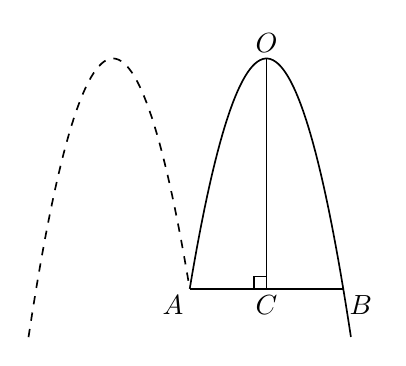
\begin{tikzpicture}[x=.65cm,y=.65cm,font=\normalsize,line width=.6pt]
\draw[dashed] plot[domain=-4.65:-1.5,samples=65] (\x,{4.5-2*(\x+3)*(\x+3)});
\draw plot[domain=-1.5:1.65,samples=65] (\x,{4.5-2*\x*\x});
\draw (-1.5,0)--(1.5,0);\draw (0,0)--(0,4.5);
\draw (-.24,0)--(-.24,.24)--(0,.24);
\node[anchor=south,inner sep=2pt] at (0,4.5) {$O$};
\node[anchor=north east,inner sep=2pt] at (-1.5,0) {$A$};
\node[anchor=north west,inner sep=2pt] at (1.5,0) {$B$};
\node[anchor=north,inner sep=2pt] at (0,0) {$C$};
\end{tikzpicture}
